\chapter{Enterprise Service Bus}
\label{cha:esb}
An Enterprise Service Bus (ESB) is a architectural pattern of the Software Oriented Architecture (SOA) Patterns, which describes a distributed computing architecture, whereby distributed services are interacting with each other via a bus system. An ESB in the industry is mostly taken as a third party middleware, which provides features for implementing integrations with the Enterprise Integration (EI) Patterns. Enterprises use third party middleware like JBoss Fuse for implementing integration services, which integrate external or internal services. JBoss Fuse is based on JBoss EAP, and bundles common frameworks used for integrations such as Camel, and is responsible for orchestration and mediation of the services. Camel provides API and implementations for the EI patterns and is widely used in the industry when it comes to integrate services\cite{CamelIA2018, Camel2015}. \\

The integration of external as well as internal services has become more important over time, especially with the appearance of cloud services like PaaS. Common ESB middleware on the market usually define the ESB as a single application, which contains all integration services, whereby all integration services share the same life-cycle. A single application representing an ESB, is contrary to its definition as a distributed architectural model, but has the advantage, that the ESB application is compiled at once, and therefore its contained services have to be consistent. Over time, the handling of the single ESB application will become inconvenient and complex, which is a common problem for a monolithic application.  \\

The increasing need for flexibility and shorter response times drives enterprises to split up their teams and integrations. This leads to separated services, which are managed as microservices, which have their own life-cycle. Decoupling of teams leads to decoupling of services, where the services need to provide a well defined and well managed public API\cite{Camel2015, RedHatAgileIntegration2017, EIP}.

\section{The need for an Enterprise Service Bus}
\label{sec:esb-need-for-esb}
Enterprises need an ESB to provide integrations between internal and external services or both, whereby the integrations are meant to provide a business value for the enterprise. An integration of an external service could enhance the reach of a customer, who now could be able to consume external partner services via the enterprise provided infrastructure or product. In the digital age, it is normal to consume a digital service like Netflix, which provides a video on demand service. Thus, integrations, an enterprise has to provide and maintain, will become more over time.

\section{Architecture}
\label{sec:esb-architecture}
Figure \vref{fig:esb-simple-architecture} illustrates the conceptional architecture of an ESB, which orchestrates and mediates integration services. A service can act either as a producer service, which gets accessed by clients, or can act as a consumer service, which acts as the client for a producer service. The ESB is responsible for orchestration, mediation, security, transformation, routing, and service discovery, whereby these aspects are covered by an ESB middleware provided frameworks and libraries. Additionally, an ESB middleware provides libraries, which help to implement Service Components under consideration of the SOA and EI Patterns\cite{EsbSoa2018, MediationESB2005}.

\begin{figure}[htbp]
	\centering
	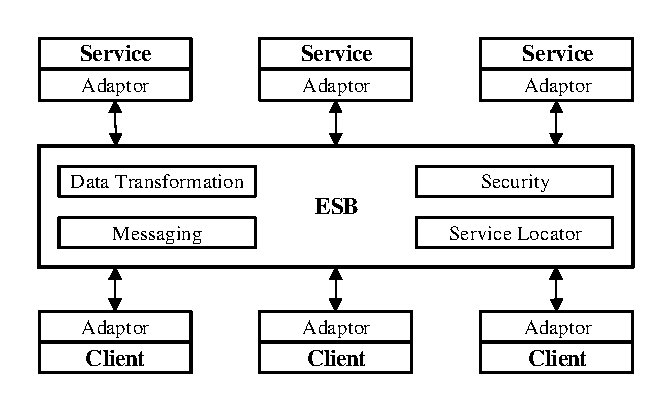
\includegraphics[scale=1]{images/esb-simple-architecture.pdf}
	\caption{Architecture of an ESB}
	\label{fig:esb-simple-architecture}
\end{figure} 

Figure \vref{fig:esb-bidirectional-integration} illustrates a bi-directional integration of services between two partner enterprises, whereby each integrated service is allowed to be consumed by the partner's customers, but only if the service is accessed via the partner's infrastructure. The ESB of the enterprises integrate the partner's provided services into their service domain, which can be accessed by their customers. For instance, an IP-TV provider can be integrated by an Internet Service Provider (ISP), to provide Internet TV for their customers.
\newpage 

\begin{figure}[htbp]
	\centering
	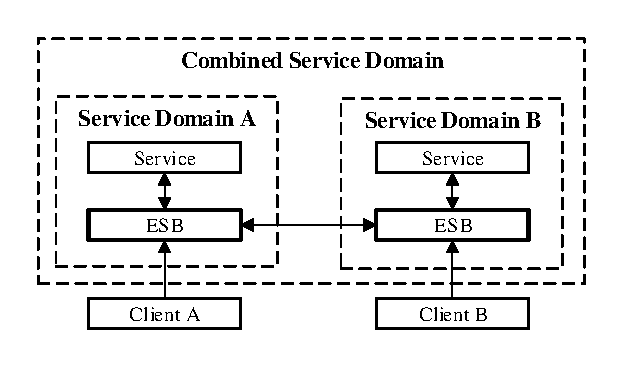
\includegraphics[scale=1]{images/esb-bidirectional-integration.pdf}
	\caption{Architecture of a bi-directional enterprise integration}
	\label{fig:esb-bidirectional-integration}
\end{figure} 

\section{Enterprise Service Bus with EAP}
\label{sec:esb-as-software}
An ESB is an architectural model for a distributed system, and has been implemented in software to provide an integration platform to developers, so that they can implement services under the consideration of the EI patterns. Before the appearance of cloud services like PaaS, ESB implementations used existing platforms such as JBoss EAP, OSGI or Karaf for the service orchestration and mediation. In case of JBoss EAP, the platform provides all libraries and frameworks developers need for implementing a service. Commonly, the services are managed within a single application, which represents the ESB application. This is a monolithic approach of organizing services, but has the advantage that the management of the services is easier, because the source code is not separated. Figure \vref{fig:esb-software-architecture} illustrates the monolithic organization of the services within a single ESB application, which is hosted on JBoss EAP.

\begin{figure}[htbp]
	\centering
	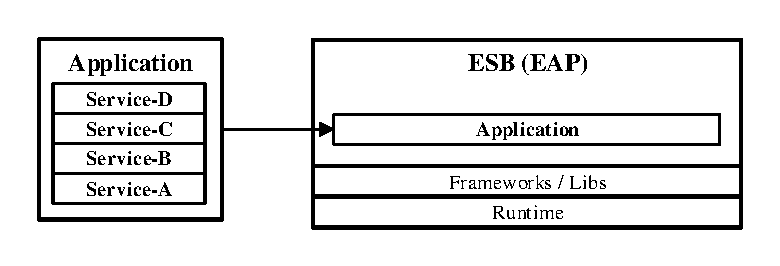
\includegraphics[scale=1]{images/esb-software-architecture.pdf}
	\caption{Monolithic ESB application}
	\label{fig:esb-software-architecture}
\end{figure} 
\ \newpage

Figure \vref{fig:esb-software-architecture} was called an ESB, but is actually not one, because the services are not distributed. Nevertheless, the industry calls such installations an ESB. The services of such an ESB application are implemented separately, but still managed within a single code base, and communicate with each other like they where on a bus system. JBoss EAP proxies the requests between the services, and therefore acts more like a message broker of an Hub and Spoke architecture, rather than acting as a bus system. The Hub and Spoke architecture was introduced, due the fact, that the count of edges of a fully connected graph requires $n / 2 * (n -1)$ edges, whereby the count of edges grows with the square of the count of nodes. A node in the graph represents a service, and an edge in the graph represents the connection between two services\cite{EIP,HubAndSpoke2003}. \\

With the appearance of cloud services such as PaaS, the PaaS platform can now take over the mediation, and security aspects of an ESB. The services can be completely separated and decoupled from each other, designed as microservices with their own life-cycle, and be managed by the cloud service. Additionally, the services are hosted in a clustered infrastructure, which allows them to be distributed among multiple nodes. The new term for this kind of ESB is IPaaS, whereby the ESB is represented by an PaaS platform such as Openshift, which provides additional tooling for implementing integration  services\cite{iPaaSP12015, iPaaSP22015}.

\section{Enterprise Service Bus with Openshift}
\label{sec:esb-as-cloud}
With the appearance and general availability of cloud services like PaaS, it is now possible to move an ESB into the cloud, whereby the cloud service takes over some aspects of the ESB middleware such as mediation and security. Openshift performs mediation via the Openshift Service abstraction, whereby multiple service instances can be present behind the Openshift Service, and the security is applied by isolating the Openshift Projects, and making services only accessible within an Openshift Project, or via an Openshift Route. The service orchestration is not needed anymore, because the services are now microservices, which need service choreography. The main difference between service orchestration and service choreography is, that the service orchestration has a local point of view and a central orchestrator component, whereby the service choreography has a global point of view and no central orchestrator component\cite{Richards2015}. \\

A main problem of existing monolithic ESB applications is the fact, that all services are managed within a single application, with one release version, and a shared life-cycle. If the ESB is represented by a cloud service, the services have to be implemented as separated services, which forces developers to separate their services into separate code bases, and to provide a proper designed and managed public API for their services. Figure \vref{fig:esb-cloud-architecture} illustrates the services of an ESB application, which runs on Openshift. \\

As discussed in the introduction of this chapter, enterprises need to separate their integrations and teams, to be faster and more responsive to business changes. Therefore, the microservice architecture, which is necessary when the ESB is represented by a cloud service, can help enterprises to become more flexible.

\begin{figure}[htbp]
	\centering
	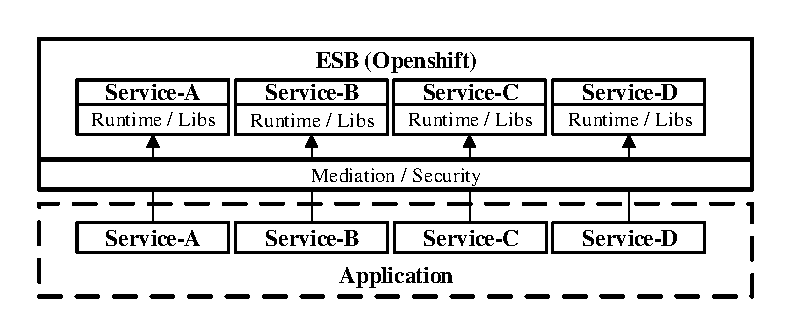
\includegraphics[scale=1]{images/esb-cloud-architecture.pdf}
	\caption{ESB application with microservices}
	\label{fig:esb-cloud-architecture}
\end{figure} 

\section{Service Integration Example}
\label{sec:esb-integration-example}
This section will discuss an example of a service integration, and how it would have been designed as part of a monolithic ESB application with JBoss Fuse based on JBoss EAP. The integration discussed in this chapter will be the base for the prototype of this thesis, which is specified in Chapter \vref{cha:esboc}. Figure \vref{fig:esb-design-services} illustrates the integration example, contained services, and involved service domains. The integration service integrates an external database with an internal application, which is consumed by a public client. How the database is allowed to be accessed is implemented in the integration service, which is the only service allowed to communicate with the external located database.

\begin{figure}[htbp]
	\centering
	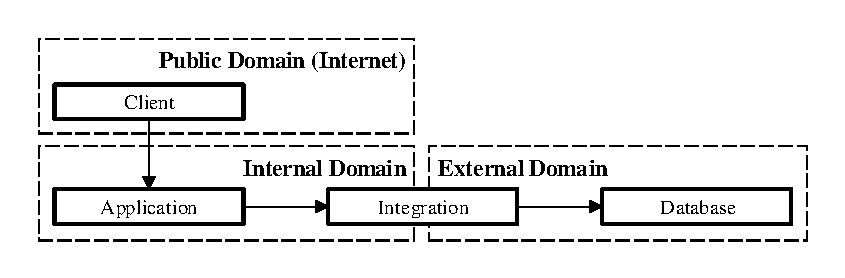
\includegraphics[scale=1]{images/esb-integration-example.pdf}
	\caption{Integration example service domains}
	\label{fig:esb-design-services}
\end{figure}
\ \newpage

Figure \vref{fig:esb-design-sca} illustrates the design of the integration in an monolithic ESB application with JBoss Fuse based on JBoss EAP and Switchyard, which provides an API for implementing a Service Component Architecture (SCA). A service within the ESB application is represented by a service component, which exposes consumable resources (Service), and calls other services (Reference)\cite{Switchyard}. 

\begin{figure}[htbp]
	\centering
	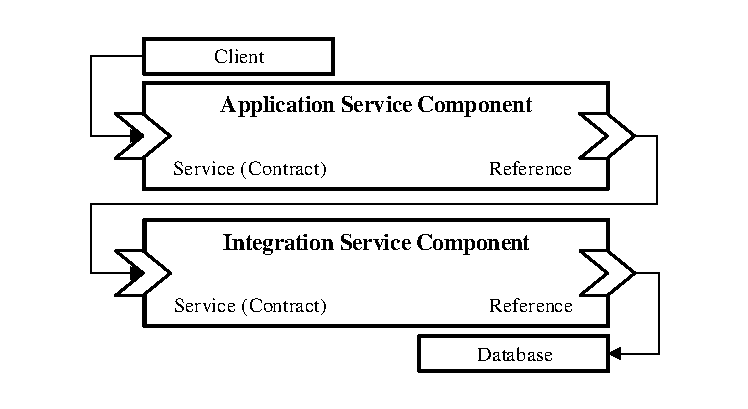
\includegraphics[scale=1]{images/esb-sca-example.pdf}
	\caption{Integration with SCA}
	\label{fig:esb-design-sca}
\end{figure}
  
ESB middleware, such as JBoss Fuse, provides frameworks and libraries, which implement the SCA patterns and provide a lightweight way of implementing service components. The service component orchestration, mediation, and security is performed by the ESB middleware. Additionally, the ESB middleware provides bindings for commonly used technologies such as REST or SOAP, which can be applied to services and references. Thus, the developers don't have to setup for instance a REST Server or REST Client anymore, but only need to provide the service contract and connection settings\cite{MicroSoa2008, Richards2015}.\\

The following chapter will specify the prototype based on the introduced example integration, and will show that an ESB can be implemented on Openshift.